\documentclass{beamer}% usefull options [handout]
\usepackage{graphicx}
\usepackage{amsmath}
%\usepackage{wrapfig}
%\useoutertheme{infolines}
\usetheme{default}% other nice themes Hannover, CambridgeUS, AnnArbor, Madrid, PaloAlto, Malmoe, Rochester 
\usecolortheme{beetle}% other options "dove"
\usefonttheme{structuresmallcapsserif}
\setbeamertemplate{items}[triangle] % other options "circle", "ball", "square"
%\setbeamertemplate{blocks}[rounded][shadow=true]
\setbeamertemplate{navigation symbols}{}
\useoutertheme[height=20pt]{sidebar}
%\setbeamercolor{normal text}{fg=white,bg=black}% inverted black background white foreground
\setbeamercolor*{palette sidebar secondary}{fg=white}

%************ Title & Author ***********************
\title[Introduction to FLCore]{An Introduction to the FLCore package}
\author{FLR Core Team}

\usepackage{Sweave}
\begin{document}

%===========================================
% INTRODUCTION
%===========================================
\section{Introduction}
%*******************************************
\begin{frame}[plain]
\titlepage
\begin{flushright}
	
\includegraphics[width=0.1\textwidth]{cc.png}
\end{flushright}
\end{frame}

%*******************************************
\begin{frame}
\frametitle{Outline}
\tableofcontents[pausesections]
\end{frame}

% some code we need 

%*******************************************
\begin{frame}
\frametitle{FLCore structure}
Follows S4 paradigm with structured data implemented as classes and several methods to apply on objects of the classes.
	\begin{itemize}
		\item<2-> Classes - empty definitions of data
		\item<3-> Objects - instances of the classes which have data following the class definition
		\item<4-> Methods - implementation of actions to be executed on objects depending on its class
		%\newline\newline
		%\item<5-> Documentation - as man pages or vignettes
		%\item<6-> Tests - code that runs during compilation to check code 
      \end{itemize}
\end{frame}

%*******************************************
\begin{frame}
  \frametitle{Inside FLCore}
	\begin{itemize}
		\item<2-> Basic classes:\newline FLArray, FLQuant, FLCohort, FLQuantPoint, FLPar
		\item<3-> Composite classes:\newline FLComp, FLBiol, FLCatch, FLFleet, FLIndex, FLMetier, FLModel, FLStock
		\item<4-> Lists of classes:\newline FLLst, FLBiols, FLCatches, FLCohorts, FLFleets, FLIndices, FLMetiers, FLQuants, FLStocks 
		\item<5-> Model class:\newline FLModel, FLGrowth, FLSR
		\item<6-> Methods
	\end{itemize}
\end{frame}

%===========================================
% BASIC CLASSES
%===========================================
\section{Basic classes}
%*******************************************
\begin{frame}[containsverbatim]
  \frametitle{Basic classes}

\scriptsize{
% latex table generated in R 2.12.0 by xtable 1.5-6 package
% Tue Nov 30 17:42:08 2010
\begin{table}[ht]
\begin{center}
\begin{tabular}{rlrllr}
  \hline
 & parent & nSlots & virtual & child & distance \\ 
  \hline
FLCohort & FLArray &   2 & FALSE &  &  \\ 
  FLQuant & FLArray &   2 & FALSE & FLQuantPoint & 1.00 \\ 
  FLQuantPoint & FLQuant &   2 & FALSE &  &  \\ 
   \hline
\end{tabular}
\end{center}
\end{table}}

\end{frame}

%*******************************************
\begin{frame}
  \frametitle{FLQuant}

Six dimensional array used to store data of a particular type (e.g. catch numbers).\newline

Dimensions are:
      \begin{enumerate}
	 \item<2-> User defined (age, length etc.)
	 \item<3-> Year
	 \item<4-> Unit (substocks, male/female)
	 \item<5-> Season
	 \item<6-> Area
	 \item<7-> Iter
      \end{enumerate}
\end{frame}

%***********************************
\begin{frame}[containsverbatim]

  \frametitle{FLQuant example}

{\tiny{
\begin{Schunk}
\begin{Sinput}
> data(ple4)
> flq <- window(landings.n(ple4), start = 1995, end = 2001)
> dimnames(flq)
\end{Sinput}
\begin{Soutput}
$age
 [1] "1"  "2"  "3"  "4"  "5"  "6"  "7"  "8"  "9"  "10"

$year
[1] "1995" "1996" "1997" "1998" "1999" "2000" "2001"

$unit
[1] "unique"

$season
[1] "all"

$area
[1] "unique"

$iter
[1] "1"
\end{Soutput}
\end{Schunk}
}}

\end{frame}

%***************************************
\begin{frame}[containsverbatim]
  \frametitle{FLQuant methods}

{\tiny{
\begin{Schunk}
\begin{Sinput}
> getClassMethods("FLQuant", "package:FLCore")
\end{Sinput}
\begin{Soutput}
  [1] "apply"          "areaMeans"      "areaSums"       "areaVars"      
  [5] "as.data.frame"  "as.FLQuant"     "barchart"       "[<-"           
  [9] "["              "bubbles"        "bwplot"         "capacity<-"    
 [13] "catch<-"        "catch.n<-"      "catch.q<-"      "catch.wt<-"    
 [17] "coerce"         "crewshare<-"    "cv"             "dimMeans"      
 [21] "dimnames<-"     "dims"           "dimSums"        "dimVars"       
 [25] "discards<-"     "discards.n<-"   "discards.sel<-" "discards.wt<-" 
 [29] "dotplot"        "effort<-"       "effshare<-"     "E"             
 [33] "fcost<-"        "fec<-"          "FLBiol"         "FLCatch"       
 [37] "FLCohort"       "FLIndex"        "FLMetier"       "FLQuant"       
 [41] "FLQuantPoint"   "FLStock"        "harvest<-"      "harvest.spwn<-"
 [45] "histogram"      "index<-"        "index.q<-"      "index.var<-"   
 [49] "iter<-"         "iterMeans"      "iters"          "iterVars"      
 [53] "jacknife"       "landings<-"     "landings.n<-"   "landings.sel<-"
 [57] "landings.wt<-"  "loglAR1"        "mat<-"          "m<-"           
 [61] "m.spwn<-"       "names"          "n<-"            "plot"          
 [65] "price<-"        "print"          "propagate"      "pv"            
 [69] "quant<-"        "quant"          "quantile"       "quantMeans"    
 [73] "quantSums"      "quantTotals"    "quantVars"      "rec<-"         
 [77] "r"              "rlnorm"         "rnorm"          "rpois"         
 [81] "rSq"            "seasonMeans"    "seasonSums"     "seasonVars"    
 [85] "sel.pattern<-"  "setPlusGroup"   "sp"             "spr0"          
 [89] "spwn<-"         "ssb<-"          "stock<-"        "stock.n<-"     
 [93] "stock.wt<-"     "stripplot"      "sweep"          "unitMeans"     
 [97] "units<-"        "units"          "unitSums"       "unitVars"      
[101] "vcost<-"        "window"         "wt<-"           "xyplot"        
[105] "yearMeans"      "yearSums"       "yearTotals"     "yearVars"      
\end{Soutput}
\end{Schunk}
}}

\end{frame}

%*******************************************
\begin{frame}[containsverbatim]
  \frametitle{FLQuantPoint}

Six dimensional array used to summarize FLQuant objects.\newline

{\tiny{
\begin{Schunk}
\begin{Sinput}
> dimnames(FLQuantPoint(flq))
\end{Sinput}
\begin{Soutput}
$age
 [1] "1"  "2"  "3"  "4"  "5"  "6"  "7"  "8"  "9"  "10"

$year
[1] "1995" "1996" "1997" "1998" "1999" "2000" "2001"

$unit
[1] "unique"

$season
[1] "all"

$area
[1] "unique"

$iter
[1] "mean"   "median" "var"    "uppq"   "lowq"  
\end{Soutput}
\end{Schunk}
}}

\end{frame}

%***************************************
\begin{frame}[containsverbatim]
  \frametitle{FLQuantPoint methods}

{\tiny{
\begin{Schunk}
\begin{Sinput}
> getClassMethods("FLQuantPoint", "package:FLCore")
\end{Sinput}
\begin{Soutput}
 [1] "[<-"      "coerce"   "lowq<-"   "lowq"     "mean"     "mean<-"  
 [7] "median<-" "median"   "plot"     "quantile" "rgamma"   "rlnorm"  
[13] "rnorm"    "show"     "summary"  "uppq<-"   "uppq"     "var<-"   
[19] "var"     
\end{Soutput}
\end{Schunk}
}}

\end{frame}

%*******************************************
\begin{frame}[containsverbatim]
  \frametitle{FLCohort}

Six dimensional array used to store cohort data.\newline

{\tiny{
\begin{Schunk}
\begin{Sinput}
> dimnames(FLCohort(flq))
\end{Sinput}
\begin{Soutput}
$age
 [1] "1"  "2"  "3"  "4"  "5"  "6"  "7"  "8"  "9"  "10"

$cohort
 [1] "1985" "1986" "1987" "1988" "1989" "1990" "1991" "1992" "1993" "1994"
[11] "1995" "1996" "1997" "1998" "1999" "2000"

$unit
[1] "unique"

$season
[1] "all"

$area
[1] "unique"

$iter
[1] "1"
\end{Soutput}
\end{Schunk}
}}

\end{frame}

%***************************************
\begin{frame}[containsverbatim]
  \frametitle{FLCohort methods}

{\tiny{
\begin{Schunk}
\begin{Sinput}
> getClassMethods("FLCohort", "package:FLCore")
\end{Sinput}
\begin{Soutput}
 [1] "bubbles"    "ccplot"     "coerce"     "dimnames<-" "dims"      
 [6] "flc2flq"    "FLCohort"   "iter<-"     "plot"       "propagate" 
[11] "xyplot"    
\end{Soutput}
\end{Schunk}
}}

\end{frame}

%*******************************************
\begin{frame}[containsverbatim]
  \frametitle{FLPar}

A two dimensional array used to store parameter's data.\newline

{\tiny{
\begin{Schunk}
\begin{Sinput}
> dimnames(new("FLPar"))
\end{Sinput}
\begin{Soutput}
$param
[1] ""

$iter
[1] "1"
\end{Soutput}
\end{Schunk}
}}

\end{frame}

%***************************************
\begin{frame}[containsverbatim]
  \frametitle{FLPar methods}

{\tiny{
\begin{Schunk}
\begin{Sinput}
> getClassMethods("FLPar", "package:FLCore")
\end{Sinput}
\begin{Soutput}
 [1] "ab"            "Arith"         "as.data.frame" "[<-"          
 [5] "["             "coerce"        "convertFLPar"  "densityplot"  
 [9] "dims"          "FLPar"         "fmle"          "histogram"    
[13] "iter<-"        "iter"          "mean"          "median"       
[17] "names<-"       "names"         "params<-"      "plot"         
[21] "propagate"     "show"          "splom"         "summary"      
[25] "sv"            "sweep"         "units<-"       "units"        
[29] "var"          
\end{Soutput}
\end{Schunk}
}}

\end{frame}

%===========================================
% COMPOSITE CLASSES
%===========================================
\section{Composite classes}
%*******************************************
\begin{frame}[containsverbatim]
  \frametitle{Composite classes}

Classes that use FLQuant classes to define their slots.

\scriptsize{
% latex table generated in R 2.12.0 by xtable 1.5-6 package
% Tue Nov 30 17:42:09 2010
\begin{table}[ht]
\begin{center}
\begin{tabular}{rlrllr}
  \hline
 & parent & nSlots & virtual & child & distance \\ 
  \hline
FLBiol & FLComp &   8 & FALSE &  &  \\ 
  FLCatch & FLComp &  13 & FALSE &  &  \\ 
  FLFleet & FLComp &   8 & FALSE &  &  \\ 
  FLIndex & FLComp &  12 & FALSE &  &  \\ 
  FLMetier & FLComp &   7 & FALSE &  &  \\ 
  FLModel.1 & FLComp &  14 & FALSE & FLSR & 1.00 \\ 
  FLModel.1.1 & FLComp &  14 & FALSE & FLGrowth & 1.00 \\ 
  FLStock & FLComp &  20 & FALSE &  &  \\ 
   \hline
\end{tabular}
\end{center}
\end{table}}

\end{frame}

%***************************************
\begin{frame}[containsverbatim]
  \frametitle{FLStock}
Represents a fish stock and comprises a number of slots.
{\tiny{
\begin{Schunk}
\begin{Sinput}
> showClass("FLStock")
\end{Sinput}
\begin{Soutput}
Class "FLStock" [package "FLCore"]

Slots:
                                                                       
Name:         catch      catch.n     catch.wt     discards   discards.n
Class:      FLQuant      FLQuant      FLQuant      FLQuant      FLQuant
                                                                       
Name:   discards.wt     landings   landings.n  landings.wt        stock
Class:      FLQuant      FLQuant      FLQuant      FLQuant      FLQuant
                                                                       
Name:       stock.n     stock.wt            m          mat      harvest
Class:      FLQuant      FLQuant      FLQuant      FLQuant      FLQuant
                                                                       
Name:  harvest.spwn       m.spwn         name         desc        range
Class:      FLQuant      FLQuant    character    character      numeric

Extends: "FLComp"
\end{Soutput}
\end{Schunk}
}}
\end{frame}

%***************************************
\begin{frame}[containsverbatim]
  \frametitle{FLStock example}
{\tiny{
\begin{Schunk}
\begin{Sinput}
> summary(ple4)
\end{Sinput}
\begin{Soutput}
An object of class "FLStock"

Name: Plaice in IV 
Description: Imported from a VPA file. ( N:\Projecten\ICES WG\Demersale werkgroep WGNSSK\2009\stock\ple-nsea\final runs\index.txt ).  Tue Jun 16 06:32:20 2009 + FLAssess:  
Range:	 min	max	pgroup	minyear	maxyear	minfbar	maxfbar 
	1	10	10	1957	2008	2	6	
Quant: age 

catch         : [ 1 52 1 1 1 1 ], units =  tonnes 
catch.n       : [ 10 52 1 1 1 1 ], units =  thousands 
catch.wt      : [ 10 52 1 1 1 1 ], units =  kg 
discards      : [ 1 52 1 1 1 1 ], units =  tonnes 
discards.n    : [ 10 52 1 1 1 1 ], units =  thousands 
discards.wt   : [ 10 52 1 1 1 1 ], units =  kg 
landings      : [ 1 52 1 1 1 1 ], units =  tonnes 
landings.n    : [ 10 52 1 1 1 1 ], units =  thousands 
landings.wt   : [ 10 52 1 1 1 1 ], units =  kg 
stock         : [ 1 52 1 1 1 1 ], units =  tonnes 
stock.n       : [ 10 52 1 1 1 1 ], units =  thousands 
stock.wt      : [ 10 52 1 1 1 1 ], units =  kg 
m             : [ 10 52 1 1 1 1 ], units =  NA 
mat           : [ 10 52 1 1 1 1 ], units =  NA 
harvest       : [ 10 52 1 1 1 1 ], units =  f 
harvest.spwn  : [ 10 52 1 1 1 1 ], units =  NA 
m.spwn        : [ 10 52 1 1 1 1 ], units =  NA 
\end{Soutput}
\end{Schunk}
}}
\end{frame}

%***************************************
\begin{frame}[containsverbatim]
  \frametitle{FLStock methods}

{\tiny{
\begin{Schunk}
\begin{Sinput}
> getClassMethods("FLStock", "package:FLCore")
\end{Sinput}
\begin{Soutput}
 [1] "as.FLBiol"       "as.FLSR"         "[<-"             "["              
 [5] "+"               "catch<-"         "catch"           "catch.n<-"      
 [9] "catch.n"         "catch.wt<-"      "catch.wt"        "coerce"         
[13] "computeCatch"    "computeDiscards" "computeLandings" "computeStock"   
[17] "dimnames<-"      "dims"            "discards<-"      "discards"       
[21] "discards.n<-"    "discards.n"      "discards.wt<-"   "discards.wt"    
[25] "expand"          "fapex"           "fbar"            "harvest<-"      
[29] "harvest"         "harvest.spwn<-"  "harvest.spwn"    "landings<-"     
[33] "landings"        "landings.n<-"    "landings.n"      "landings.wt<-"  
[37] "landings.wt"     "mat<-"           "mat"             "m<-"            
[41] "m"               "m.spwn<-"        "m.spwn"          "name"           
[45] "plot"            "qapply"          "range"           "rec"            
[49] "r"               "setPlusGroup"    "sp"              "spr0"           
[53] "ssb"             "ssbpurec"        "stock<-"         "stock"          
[57] "stock.n<-"       "stock.n"         "stock.wt<-"      "stock.wt"       
[61] "summary"         "survprob"        "trim"            "tsb"            
\end{Soutput}
\end{Schunk}
}}

\end{frame}

%%***************************************
\begin{frame}
  \frametitle{FLStock plot}

\includegraphics{intro2FLCore-015}

\end{frame}

%%***************************************
\begin{frame}[containsverbatim]
  \frametitle{FLBiol}
Represents a biological population
{\tiny{
\begin{Schunk}
\begin{Sinput}
> showClass("FLBiol")
\end{Sinput}
\begin{Soutput}
Class "FLBiol" [package "FLCore"]

Slots:
                                                                            
Name:          n         m        wt       fec      spwn      name      desc
Class:   FLQuant   FLQuant   FLQuant   FLQuant   FLQuant character character
                
Name:      range
Class:   numeric

Extends: "FLComp"
\end{Soutput}
\end{Schunk}
}}

\end{frame}

%***************************************
\begin{frame}[containsverbatim]
  \frametitle{FLBiol example}
{\tiny{
\begin{Schunk}
\begin{Sinput}
> summary(flbiol)
\end{Sinput}
\begin{Soutput}
An object of class "FLBiol"

Name: Plaice in IV 
Description: Imported from a VPA file. ( N:\Projecten\ICES WG\Demersale werkgroep WGNSSK\2009\stock\ple-nsea\final runs\index.txt ).  Tue Jun 16 06:32:20 2009 + FLAssess:  
Range:	 min	max	pgroup	minyear	maxyear	minfbar	maxfbar 
	1	10	10	1957	2008	2	6	
Quant: age 

n             : [ 10 52 1 1 1 1 ], units =  thousands 
m             : [ 10 52 1 1 1 1 ], units =  NA 
wt            : [ 10 52 1 1 1 1 ], units =  kg 
fec           : [ 10 52 1 1 1 1 ], units =  NA 
spwn          : [ 10 52 1 1 1 1 ], units =  NA 
\end{Soutput}
\end{Schunk}
}}
\end{frame}

%***************************************
\begin{frame}[containsverbatim]
  \frametitle{FLBiol methods}

{\tiny{
\begin{Schunk}
\begin{Sinput}
> getClassMethods("FLBiol", "package:FLCore")
\end{Sinput}
\begin{Soutput}
 [1] "as.FLBiol"     "as.FLSR"       "catch.n"       "coerce"       
 [5] "computeStock"  "fbar"          "fec<-"         "fec"          
 [9] "harvest"       "leslie"        "mean.lifespan" "m<-"          
[13] "m"             "n<-"           "n"             "plot"         
[17] "rec"           "r"             "setPlusGroup"  "spwn<-"       
[21] "spwn"          "ssb"           "ssn"           "summary"      
[25] "survprob"      "tsb"           "wt<-"          "wt"           
\end{Soutput}
\end{Schunk}
}}

\end{frame}

%***************************************
\begin{frame}
  \frametitle{FLBiol plot}

\includegraphics{intro2FLCore-019}

\end{frame}

%***************************************
\begin{frame}[containsverbatim]
  \frametitle{FLIndex}
Represents a index (e.g. index of abundance from a survey)
{\tiny{
\begin{Schunk}
\begin{Sinput}
> showClass("FLIndex")
\end{Sinput}
\begin{Soutput}
Class "FLIndex" [package "FLCore"]

Slots:
                                                                       
Name:          type distribution        index    index.var      catch.n
Class:    character    character      FLQuant      FLQuant      FLQuant
                                                                       
Name:      catch.wt       effort  sel.pattern      index.q         name
Class:      FLQuant      FLQuant      FLQuant      FLQuant    character
                                
Name:          desc        range
Class:    character      numeric

Extends: "FLComp"
\end{Soutput}
\end{Schunk}
}}

\end{frame}

%***************************************
\begin{frame}[containsverbatim]
  \frametitle{FLIndex example}
{\tiny{
\begin{Schunk}
\begin{Sinput}
> summary(ple4.index)
\end{Sinput}
\begin{Soutput}
An object of class "FLIndex"

Name: BTS-Isis 
Description: Plaice in IV . Imported from VPA file. 
Range:	 min	max	pgroup	minyear	maxyear	startf	endf 
	1	8	NA	1985	2008	0.66	0.75	
Type :   
Distribution :   
Quant: age 

index         : [ 8 24 1 1 1 1 ], units =  NA 
index.var     : [ 8 24 1 1 1 1 ], units =  NA 
catch.n       : [ 8 24 1 1 1 1 ], units =  NA 
catch.wt      : [ 8 24 1 1 1 1 ], units =  NA 
effort        : [ 1 24 1 1 1 1 ], units =  NA 
sel.pattern   : [ 8 24 1 1 1 1 ], units =  NA 
index.q       : [ 8 24 1 1 1 1 ], units =  NA 
\end{Soutput}
\end{Schunk}
}}
\end{frame}

%***************************************
\begin{frame}[containsverbatim]
  \frametitle{FLIndex methods}

{\tiny{
\begin{Schunk}
\begin{Sinput}
> getClassMethods("FLIndex", "package:FLCore")
\end{Sinput}
\begin{Soutput}
 [1] "["             "catch.n<-"     "catch.n"       "catch.wt<-"   
 [5] "catch.wt"      "coerce"        "computeCatch"  "dims"         
 [9] "effort<-"      "effort"        "index<-"       "index"        
[13] "index.q<-"     "index.q"       "index.var<-"   "index.var"    
[17] "plot"          "sel.pattern<-" "sel.pattern"   "summary"      
[21] "trim"          "type<-"        "type"         
\end{Soutput}
\end{Schunk}
}}

\end{frame}

%***************************************
\begin{frame}
  \frametitle{FLBiol plot}

\includegraphics{intro2FLCore-023}

\end{frame}

%***************************************
\begin{frame}
  \frametitle{FLFleet}
A more complicated class with three levels: Fleet, Metier and Catch
   \begin{center}
      \includegraphics[width=1\textwidth]{FLFleet.png}
   \end{center}
\end{frame}

%***************************************
\begin{frame}[containsverbatim]
  \frametitle{FLFleet}
{\tiny{
\begin{Schunk}
\begin{Sinput}
> showClass("FLFleet")
\end{Sinput}
\begin{Soutput}
Class "FLFleet" [package "FLCore"]

Slots:
                                                                            
Name:     effort     fcost  capacity crewshare   metiers      name      desc
Class:   FLQuant   FLQuant   FLQuant   FLQuant FLMetiers character character
                
Name:      range
Class:   numeric

Extends: "FLComp"
\end{Soutput}
\end{Schunk}
}}

\end{frame}

%***************************************
\begin{frame}[containsverbatim]
  \frametitle{FLFleet example}
{\tiny{
\begin{Schunk}
\begin{Sinput}
> summary(bt4)
\end{Sinput}
\begin{Soutput}
An object of class "FLFleet"

Name: beam trawl fleet 
Description: Example of an FLFleet 
Range:	 min	max	pgroup	minyear	maxyear 
	0	0	NA	1957	2001	
Quant: age 

effort        : [ 1 45 1 1 1 1 ], units =  NA 
fcost         : [ 1 45 1 1 1 1 ], units =  NA 
capacity      : [ 1 45 1 1 1 1 ], units =  NA 
crewshare     : [ 1 45 1 1 1 1 ], units =  NA 

Metiers:  
	 TBB :
		 ple : [ 15 45 1 1 1 1 ]
		 sol : [ 10 45 1 1 1 1 ]
\end{Soutput}
\end{Schunk}
}}
\end{frame}

%***************************************
\begin{frame}[containsverbatim]
  \frametitle{FLFleet methods}

{\tiny{
\begin{Schunk}
\begin{Sinput}
> getClassMethods("FLFleet", "package:FLCore")
\end{Sinput}
\begin{Soutput}
 [1] "as.data.frame"   "as.FLIndex"      "["               "[["             
 [5] "capacity<-"      "capacity"        "catches"         "catch"          
 [9] "catchNames"      "catch.n"         "catch.q<-"       "catch.q"        
[13] "catch.sel"       "catch.wt"        "coerce"          "computeCatch"   
[17] "computeDiscards" "computeLandings" "crewshare<-"     "crewshare"      
[21] "dims"            "discards<-"      "discards"        "discards.n<-"   
[25] "discards.n"      "discards.sel<-"  "discards.sel"    "discards.wt<-"  
[29] "discards.wt"     "effort<-"        "effort"          "effshare"       
[33] "fcost<-"         "fcost"           "FLFleet"         "iter"           
[37] "landings<-"      "landings"        "landings.n<-"    "landings.n"     
[41] "landings.sel<-"  "landings.sel"    "landings.wt<-"   "landings.wt"    
[45] "metier<-"        "metier"          "metiers<-"       "metiers"        
[49] "price<-"         "price"           "propagate"       "revenue"        
[53] "summary"         "trim"            "vcost"           "window"         
\end{Soutput}
\end{Schunk}
}}

\end{frame}



%===========================================
% LIST CLASSES
%===========================================
\section{List classes}
%*******************************************
\begin{frame}[containsverbatim]
  \frametitle{List classes}

\scriptsize{
% latex table generated in R 2.12.0 by xtable 1.5-6 package
% Tue Nov 30 17:42:17 2010
\begin{table}[ht]
\begin{center}
\begin{tabular}{rlrllr}
  \hline
 & parent & nSlots & virtual & child & distance \\ 
  \hline
FLBiols & FLlst &   4 & FALSE &  &  \\ 
  FLCatches & FLlst &   4 & FALSE &  &  \\ 
  FLCohorts & FLlst &   4 & FALSE &  &  \\ 
  FLFleets & FLlst &   4 & FALSE &  &  \\ 
  FLIndices & FLlst &   4 & FALSE &  &  \\ 
  FLMetiers & FLlst &   4 & FALSE &  &  \\ 
  FLQuants & FLlst &   4 & FALSE &  &  \\ 
  FLStocks & FLlst &   4 & FALSE &  &  \\ 
   \hline
\end{tabular}
\end{center}
\end{table}}

\end{frame}


%===========================================
% MODEL CLASSES
%===========================================
\section{Model classes}
%*******************************************
\begin{frame}[containsverbatim]
  \frametitle{Model classes}

\scriptsize{
% latex table generated in R 2.12.0 by xtable 1.5-6 package
% Tue Nov 30 17:42:17 2010
\begin{table}[ht]
\begin{center}
\begin{tabular}{rlrllr}
  \hline
 & parent & nSlots & virtual & child & distance \\ 
  \hline
FLGrowth & FLModel &  15 & FALSE &  &  \\ 
  FLSR & FLModel &  18 & FALSE &  &  \\ 
   \hline
\end{tabular}
\end{center}
\end{table}}

\end{frame}

%************ Frame 14***********************
%\begin{frame}[containsverbatim]
%  \frametitle{FLSR}
%Class for fitting stock-recruitment relationships.  Extends FLModel.
%{\tiny{
%<<results=verbatim,echo=TRUE>>=
%showClass("FLSR")
%@ %def 
%}}
%\end{frame}
%
%************ Frame 14***********************
\begin{frame}[containsverbatim]
  \frametitle{FLSR}
Class for fitting stock-recruitment relationships.  Extends FLModel.
{\tiny{
\begin{Schunk}
\begin{Sinput}
> data(nsher)
> summary(nsher)
\end{Sinput}
\begin{Soutput}
An object of class "FLSR"

Name: Autumn spawning herring in IV, V  3/4/2005 14:46 
Description: 'rec' and 'ssb' slots obtained from a 'FLStock' object 
Range:	  
		
Quant: age 

rec           : [ 1 45 1 1 1 1 ], units =  NA 
ssb           : [ 1 45 1 1 1 1 ], units =  NA 
residuals     : [ 1 45 1 1 1 1 ], units =  NA NA 
fitted        : [ 1 45 1 1 1 1 ], units =  NA 

Model: 	rec ~ a * ssb * exp(-b * ssb)
<environment: 0x560f3e0>
Parameters: 
    params
iter     a        b
   1 119.4 0.009027

Log-likelihood:  16.352(0) 
Variance-covariance:    
               a            b
  a 258.66388793 1.838394e-02
  b   0.01838394 2.002586e-06
\end{Soutput}
\end{Schunk}
}}
\end{frame}

%********************************************
%\begin{frame}
%  \frametitle{FLR and plots}
%      \begin{itemize}
%	 \item plot and lattice plots
%	 \item FLEDA
%      \end{itemize}
%\end{frame}
%********************************************
\begin{frame}[plain]
  \frametitle{The FLSR plot}
%@ 
%<<FLSR,echo=F,fig=T>>=
%plot(nsher)
%@ %def 
   \begin{center}
      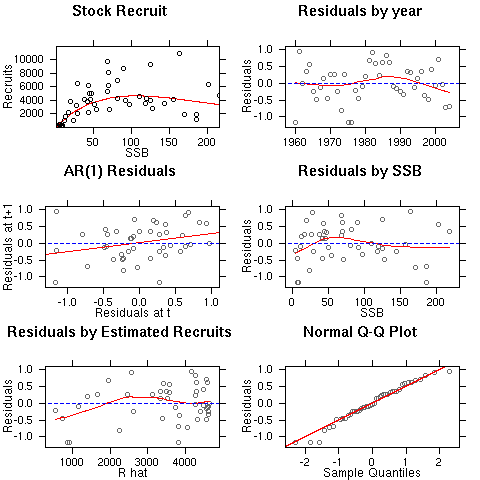
\includegraphics[width=1\textwidth]{FLSR_plot.png}
   \end{center}
\end{frame}

%A more complicated class with three levels: Fleet, Metier and Catch
%   \begin{center}
%      \includegraphics[width=1\textwidth]{/home/fas00/Work/Courses/Bergen/Presentation/fleet/FLFleet.png}
%   \end{center}
%********************************************
%\begin{frame}[plain]
%  \frametitle{FLEDA}
%@ 
%<<results=hide,echo=FALSE>>=
%library(FLEDA)
%ple4sex.spay <- spay(catch.n(ple4sex))
%# fine tune 
%ttl <- list(label="Standardized catch proportion at age for Plaice in IV", cex=1)
%yttl <- list(label="age", cex=0.8)
%xttl <- list(cex=0.8)
%ax <- list(cex=0.7)
%@
%%\end{frame}
%
%%\begin{frame}[plain]
%<<bubbles,echo=F,fig=T>>=
%# plot
%print(bubbles(age~year|unit, ple4sex.spay,  main=ttl, ylab=yttl, xlab=xttl, scales=ax, bub.scale=5))
%@ %def 
%\end{frame}
%
%************ Frame 15***********************
\begin{frame}
  \frametitle{Slot accessors}
      \begin{itemize}
	 \item<2-> Try to avoid using @ to access slots
	 \item<3-> Use accessors instead
	 \item<4-> e.g. landings.n(stock) not stock@landings.n
	 \item<5-> Protects against internal changes
	 \item<6-> e.g. catch slots removed from FLCatch
	 \item<7-> But accessor catch() still works
      \end{itemize}
\end{frame}
\end{document}

